\documentclass[hidelinks,12pt]{article}
\usepackage[utf8]{inputenc}
\usepackage[table,xcdraw]{xcolor}
\usepackage{mathtools}
\usepackage{amsthm}
\usepackage{amsmath}
\usepackage{amsfonts}
\usepackage{amssymb}
\usepackage{centernot}
\usepackage{marvosym}
\usepackage{enumitem}
\usepackage{hyperref}
\setcounter{tocdepth}{1}
\let\marvosymLightning\Lightning
\newtheorem{theorem}{Theorem}
\newtheorem{corollary}{Corollary}[theorem]
\newtheorem*{remark}{Remark}
\renewcommand\qedsymbol{QED}
\newcommand{\N}{\mathbb{N}}
\newcommand{\Z}{\mathbb{Z}}
\newcommand{\divby}{%
  \mathrel{\text{\vbox{\baselineskip.65ex\lineskiplimit0pt\hbox{.}\hbox{.}\hbox{.}}}}%
  }
\newcommand{\notdivby}{\centernot\divby}
\title{\scalebox{2}{Math 531 Homework 2}}
\author{\scalebox{1.5}{Theo Koss}}
\date{February 2021}
\begin{document}
\graphicspath{{/home/theo/Documents/GitHub/Math-Homeworks/Math 531/Random/}}
\maketitle
\section{Section 1.3}
\begin{itemize}
    \item Problem 4: Solve: $20x\equiv12\mod{72}$.$$20x=12+72q;q=-1,x=[-3]$$
    \item Problem 5: Solve: $25x\equiv45\mod{60}$.$$25x=45+60q;q=-2,x=[-3]$$
    \item Problem 7: Find additive orders of:\begin{enumerate}[label=\alph*.]
        \item $8\mod{12}:\quad3$
        \item $7\mod{12}:\quad12$
        \item $21\mod{28}:\quad3$
        \item $12\mod{18}:\quad3$
    \end{enumerate}
    \item Problem 27: Let $p$ be prime and $a,b\in\Z$. Prove, $$(a+b)^p\equiv a^p+b^p\mod{p}$$
    \begin{proof}
    By the Binomial Thm., it holds that:$$(a+b)^p=\sum_{k=0}^{p}{p\choose k}a^{k}b^{p-k}$$
Where ${p \choose k}=\frac{p!}{k!(p-k)!}$.
Then it is easy to see that $$k=0,p\Longrightarrow{p \choose k}=1$$Suppose $k\in\{1,2,...,p-1\}$ Then $${p \choose k}=\frac{p!}{k!(p-k)!}=p\cdot{l_k}$$ for some $l_{k}\in\mathbb{Z}$.
Then, by definition, ${p \choose k}\equiv0\mod{p}$.
\newline Thus, all ${p \choose k}$ such that $k\in\{1,2,...,p-1\}$ are equivalent to $0\mod{p}$.
Therefore, $(a+b)^p=a^p+b^p$ for prime $p$ and $a,b\in\mathbb{Z}$. 
    \end{proof}
\end{itemize}
\section{Section 1.4}
\begin{itemize}
    \item Problem 2: Multiplication tables:\newline\scalebox{.175}{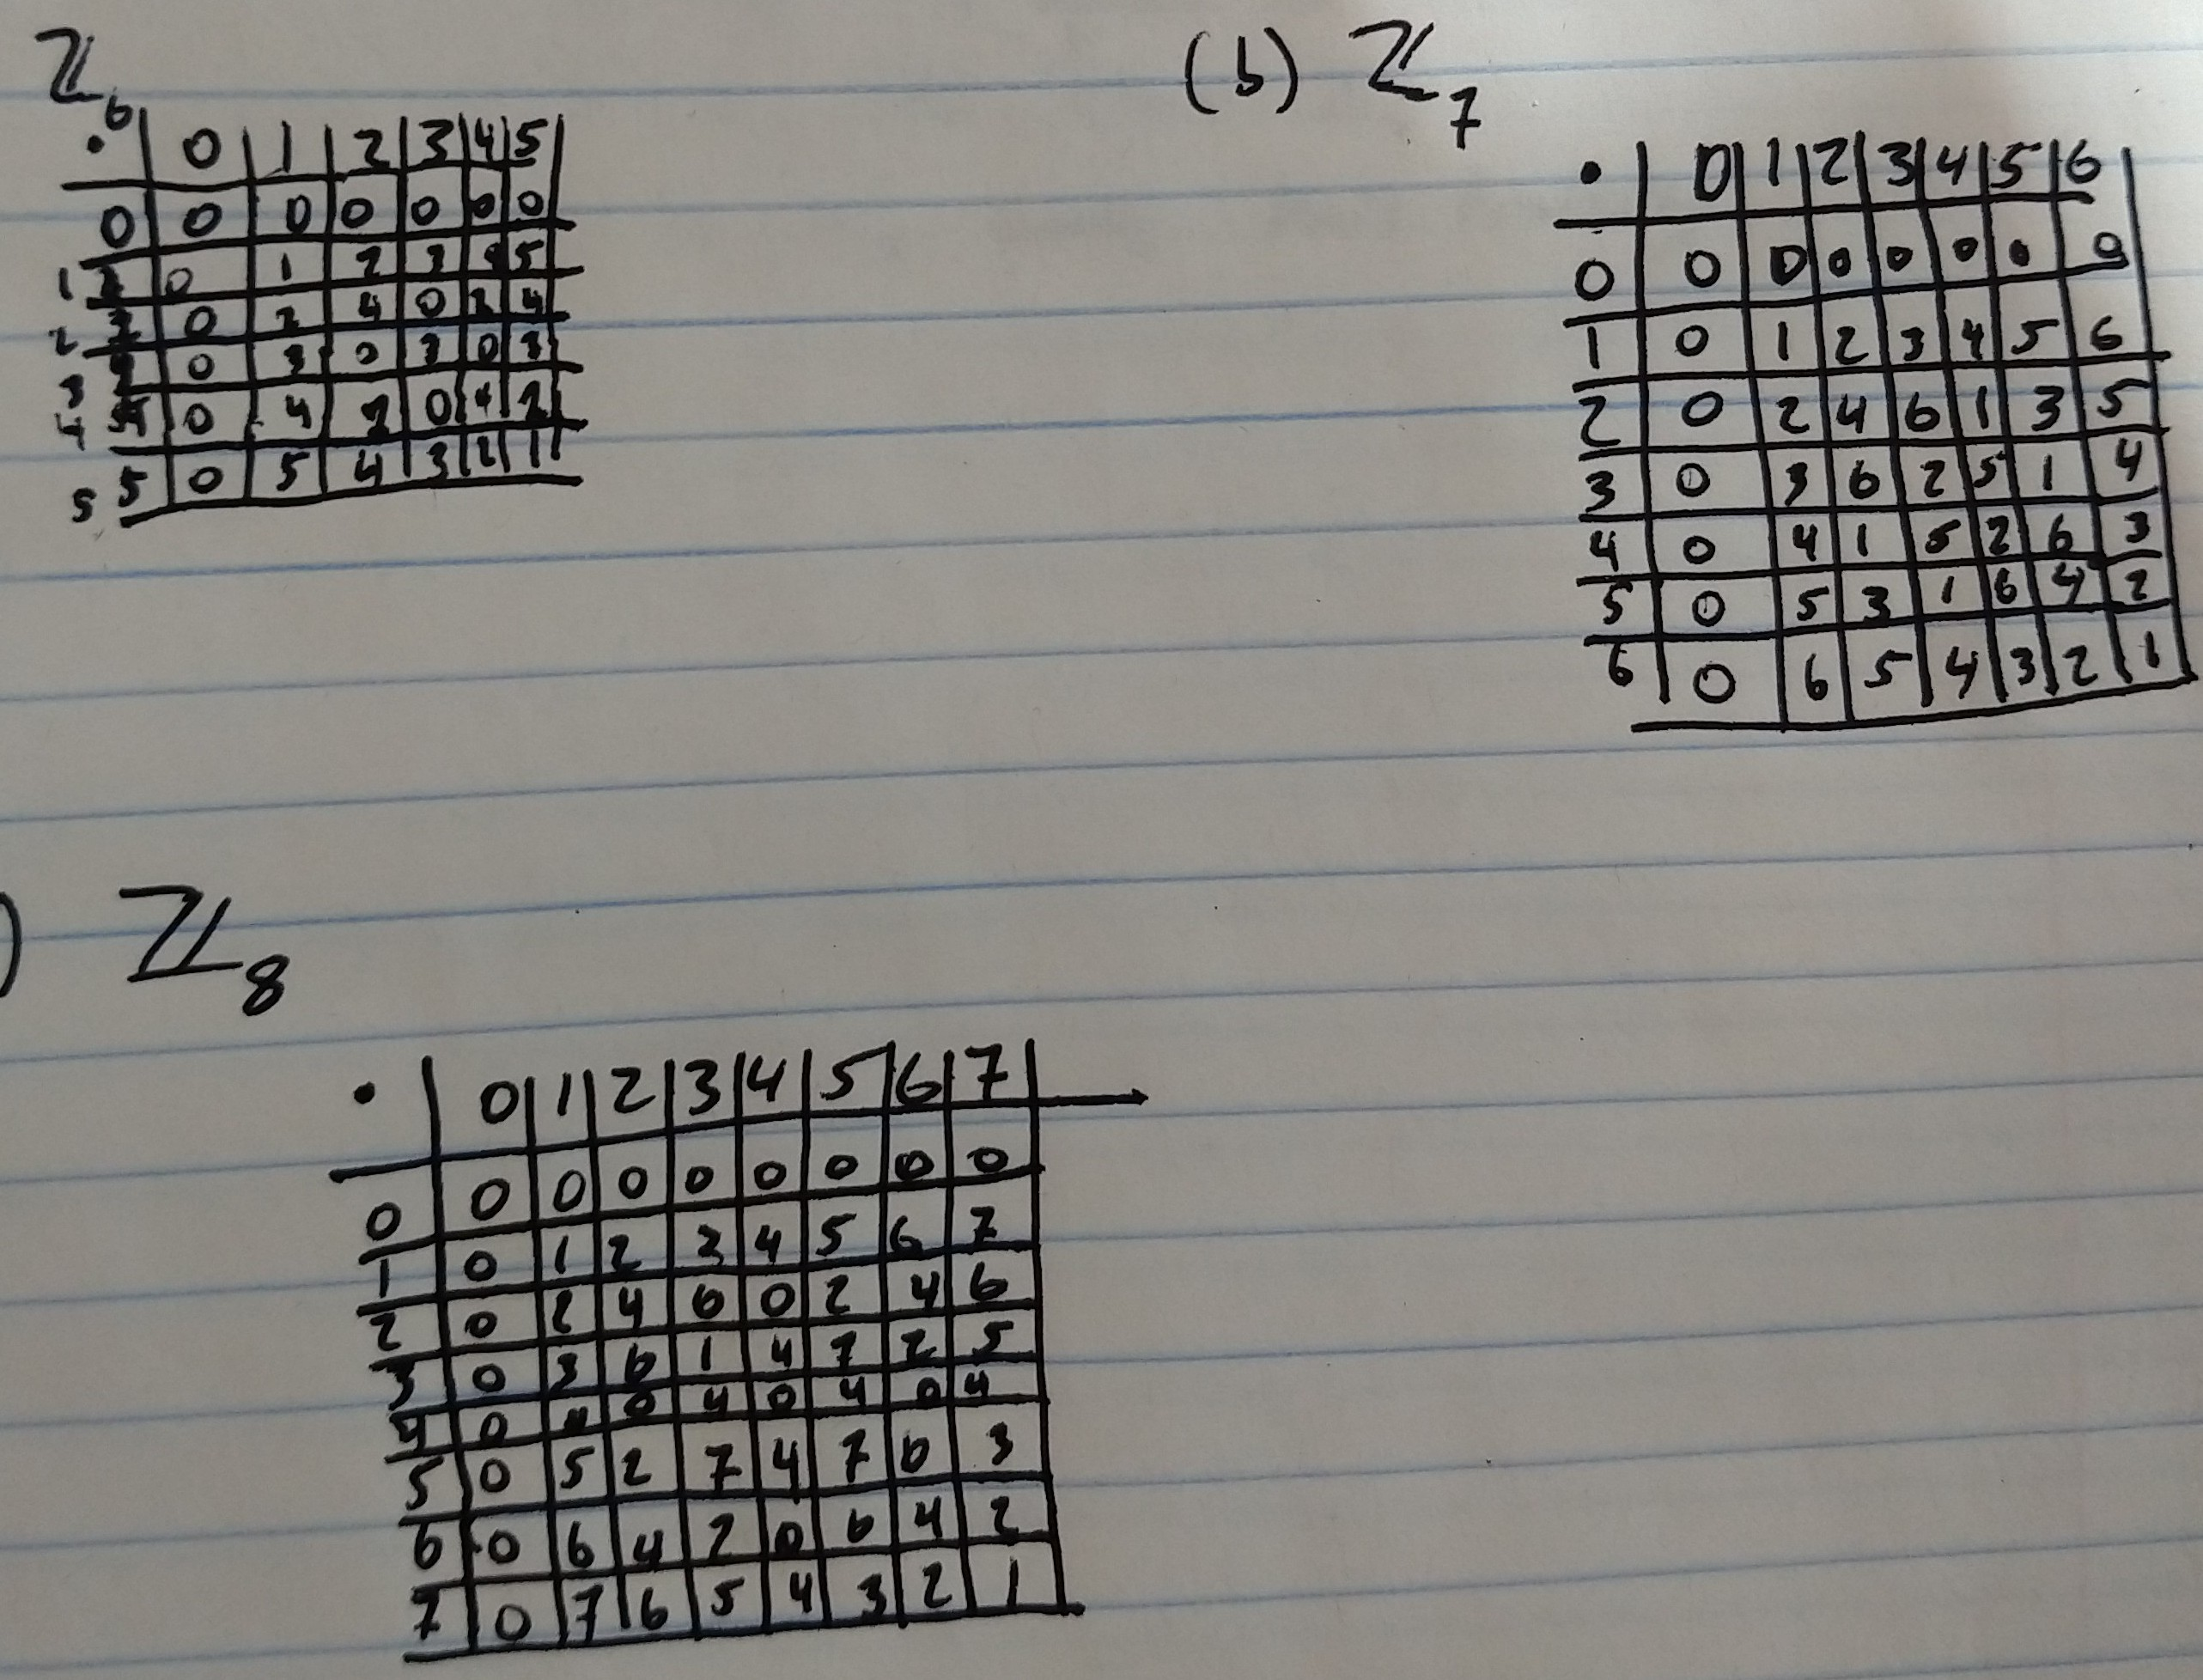
\includegraphics{MultTables}}
    \item Problem 9: \begin{enumerate}[label=\alph*.]
        \item Find multiplicative orders of $[5]$ and $[7]$ in $\Z^x_{16}$.
\newline $5^4\equiv1\mod{16};7^2\equiv1\mod{16}$. Mult. orders, 4 and 2 respectively.
\item Find multiplicative orders of $[2]$ and $[5]$ in $\Z^x_{17}$.\newline $2^8\equiv1\mod{17};5^{16}\equiv1\mod{17}$.
    \end{enumerate}
    \item Problem 12: In $\Z_9^x$ each element is equal to a power of $[2]$. Can you find a congruence class in $\Z_8^x$ such that each element of $\Z_8^x$ is equal to some power of that class? Answer the same question for $\Z_7^x$.\newline $[3]\in\Z_8^x$ is a generator. As is $[3]\in\Z_7^x$.
    \item Problem 13: Show that $\Z_{10}^x$ and $\Z_{11}^x$ are cyclic, but $\Z_{12}^x$ is not.\begin{proof}
    By \href{https://en.wikipedia.org/wiki/Multiplicative_group_of_integers_modulo_n#Cyclic_case}{\color{blue}some guy on wikipedia}, The group $\Z_n^x$ is cyclic iff $n\in\{1,2,4,p^k,2p^k\}$. Where $p$ is an odd prime and $k\in\N$. Since $10=2\cdot\underbrace{5}_{\text{odd prime}}$ and $11=\underbrace{11^1}_{\text{odd prime}}$, $\Z_{10}^x$ and $\Z_{11}^x$ are cyclic. However, $12$ is not of that form, therefore it is not cyclic. (I call this one, ``proof by wikipedia.")
    \end{proof}
\end{itemize}
\end{document}
